\documentclass[11pt,]{article}
\usepackage[left=1in,top=1in,right=1in,bottom=1in]{geometry}
\newcommand*{\authorfont}{\fontfamily{phv}\selectfont}
\usepackage[]{mathpazo}


  \usepackage[T1]{fontenc}
  \usepackage[utf8]{inputenc}



\usepackage{abstract}
\renewcommand{\abstractname}{}    % clear the title
\renewcommand{\absnamepos}{empty} % originally center

\renewenvironment{abstract}
 {{%
    \setlength{\leftmargin}{0mm}
    \setlength{\rightmargin}{\leftmargin}%
  }%
  \relax}
 {\endlist}

\makeatletter
\def\@maketitle{%
  \newpage
%  \null
%  \vskip 2em%
%  \begin{center}%
  \let \footnote \thanks
    {\fontsize{18}{20}\selectfont\raggedright  \setlength{\parindent}{0pt} \@title \par}%
}
%\fi
\makeatother




\setcounter{secnumdepth}{3}

\usepackage{longtable,booktabs}

\usepackage{graphicx,grffile}
\makeatletter
\def\maxwidth{\ifdim\Gin@nat@width>\linewidth\linewidth\else\Gin@nat@width\fi}
\def\maxheight{\ifdim\Gin@nat@height>\textheight\textheight\else\Gin@nat@height\fi}
\makeatother
% Scale images if necessary, so that they will not overflow the page
% margins by default, and it is still possible to overwrite the defaults
% using explicit options in \includegraphics[width, height, ...]{}
\setkeys{Gin}{width=\maxwidth,height=\maxheight,keepaspectratio}

\title{Análisis Morfométrico de la Microcuenca Caña, República Dominicana,
Aplicando Tecnología Geoespacial de Código Abierto.  }



\author{\Large Cinthia Amalia Vandepool Candelario\vspace{0.05in} \newline\normalsize\emph{Estudiante de Geografía mención Recursos Naturales y Ecoturismo,
Universidad Autónoma de Santo Domingo (UASD)}  }


\date{}

\usepackage{titlesec}

\titleformat*{\section}{\normalsize\bfseries}
\titleformat*{\subsection}{\normalsize\itshape}
\titleformat*{\subsubsection}{\normalsize\itshape}
\titleformat*{\paragraph}{\normalsize\itshape}
\titleformat*{\subparagraph}{\normalsize\itshape}

\titlespacing{\section}
{0pt}{36pt}{0pt}
\titlespacing{\subsection}
{0pt}{36pt}{0pt}
\titlespacing{\subsubsection}
{0pt}{36pt}{0pt}





\newtheorem{hypothesis}{Hypothesis}
\usepackage{setspace}

\makeatletter
\@ifpackageloaded{hyperref}{}{%
\ifxetex
  \PassOptionsToPackage{hyphens}{url}\usepackage[setpagesize=false, % page size defined by xetex
              unicode=false, % unicode breaks when used with xetex
              xetex]{hyperref}
\else
  \PassOptionsToPackage{hyphens}{url}\usepackage[unicode=true]{hyperref}
\fi
}

\@ifpackageloaded{color}{
    \PassOptionsToPackage{usenames,dvipsnames}{color}
}{%
    \usepackage[usenames,dvipsnames]{color}
}
\makeatother
\hypersetup{breaklinks=true,
            bookmarks=true,
            pdfauthor={Cinthia Amalia Vandepool Candelario (Estudiante de Geografía mención Recursos Naturales y Ecoturismo,
Universidad Autónoma de Santo Domingo (UASD))},
             pdfkeywords = {morfometría fluvial, modelo digital de elevación, red de drenaje, razón
de bifurcación},  
            pdftitle={Análisis Morfométrico de la Microcuenca Caña, República Dominicana,
Aplicando Tecnología Geoespacial de Código Abierto.},
            colorlinks=true,
            citecolor=blue,
            urlcolor=blue,
            linkcolor=magenta,
            pdfborder={0 0 0}}
\urlstyle{same}  % don't use monospace font for urls

% set default figure placement to htbp
\makeatletter
\def\fps@figure{htbp}
\makeatother

\usepackage{pdflscape} \newcommand{\blandscape}{\begin{landscape}}
\newcommand{\elandscape}{\end{landscape}}


% add tightlist ----------
\providecommand{\tightlist}{%
\setlength{\itemsep}{0pt}\setlength{\parskip}{0pt}}

\begin{document}
	
% \pagenumbering{arabic}% resets `page` counter to 1 
%
% \maketitle

{% \usefont{T1}{pnc}{m}{n}
\setlength{\parindent}{0pt}
\thispagestyle{plain}
{\fontsize{18}{20}\selectfont\raggedright 
\maketitle  % title \par  

}

{
   \vskip 13.5pt\relax \normalsize\fontsize{11}{12} 
\textbf{\authorfont Cinthia Amalia Vandepool Candelario} \hskip 15pt \emph{\small Estudiante de Geografía mención Recursos Naturales y Ecoturismo,
Universidad Autónoma de Santo Domingo (UASD)}   

}

}








\begin{abstract}

    \hbox{\vrule height .2pt width 39.14pc}

    \vskip 8.5pt % \small 

\noindent Resumen del manuscrito


\vskip 8.5pt \noindent \emph{Keywords}: morfometría fluvial, modelo digital de elevación, red de drenaje, razón
de bifurcación \par

    \hbox{\vrule height .2pt width 39.14pc}



\end{abstract}


\vskip 6.5pt


\noindent  \section{Introducción}\label{introducciuxf3n}

A lo largo del último siglo se ha reducido la dificultad para realizar
análisis espaciales gracias a los novedosos avances tecnológicos, el
desarrollo de los Sistemas de Información Geográfica (SIG) ha
simplificado el arduo trabajo que suponía llevar acabo análisis
espaciales, aunque a pesar de todas las herramientas disponibles la
República Dominicana aún está pasos por detrás de muchos países en
especial en lo relacionado a los análisis de morfometría fluvial,
situación lamentable ya que la isla posee innumerables cursos fluviales
permitiéndole ocupar un lugar privilegiado en este siglo, ya que, cada
día más país sufren por la escases de agua dulce potable.

La cuenca hidrográfica a analizar en esta investigación es la
Microcuenca Caña, perteneciente a la Subcuenca del Rio Macasía, ubicada
en el extremo suroeste de la República Dominicana, dicho análisis se
realizará basándonos en datos preexistentes a partir de un \emph{modelo
digital de elevación (DEM)}, el cual es un modelo simbólico, de
estructura numérica y digital que pretende representar la distribución
espacial de la elevación del terreno, siendo la altura una variable
escalar que se distribuye en un espacio bi-dimensional (Burgos \&
Salcedo (2014)).

La morfometría fluvial se encarga de analizar los parámetros
morfométricos de una cuenca hidrográfica, tales como, la red de drenaje,
la pendiente, la forma, el orden de la red y demás aspectos físicos.(@)
Entendiendo que la cuenca hidrográfica es ese sistema o unidad
geográfica e hidrológica formada por un rio principal y todo el
territorio entre el origen del rio y su desembocadura, interactuando en
este espacio diversos factores bióticos y abióticos.

El aspecto general de una cuenca se entiende como la forma en la que se
distribuyen los cursos de agua, esta forma depende principalmente de la
gravedad y la pendiente. Diversos autores ha establecido métodos tanto
cualitativos como cuantitativos para determinar la forma de la cuenca,
además de que han establecido clasificaciones para denominar a las
cuencas con formas similares (ej: Dendrítica); Cuando nos referimos a la
red de drenaje de una cuenca estamos refiriéndonos a la relación entre
la longitud total de los cursos fluviales de todos los órdenes y el área
de la cuenca, esta variable nos permitirá establecer las características
litológicas del área de estudio (Elorza (2008)).

Además, debemos tomar en cuenta, que el orden de red de los cursos de
una cuenca indica el grado de ramificación de la red fluvial; existen
distintos métodos para jerarquizar los cursos de una red pero los dos
más conocidos y utilizados son el método de Strahler (1952) y el de
Horton (1945), gracias a esta jerarquización se puede entender mejor el
comportamiento del sistema de drenaje de la cuenca, además de que se
puede obtener la razón de bifurcación descrita por Horton como la
relación entre el número de cursos de un orden y número de cursos de
orden más alto, esta propiedad es condicionada por la forma que presenta
la cuenca (Elorza (2008) Lux Cardona (2016) Ibañez Asensio, Moreno
Ramón, \& Gisbert Blanquer (2011)).

Gutierrez-Elorza (2008), sostiene que el perfil longitudinal de una rio
es la línea obtenida a partir de las diferencias de alturas desde su
afloramiento hasta desembocar en otro cuerpo de agua, este perfil es
cóncavo, aunque no todos los ríos lo presentan de manera clara debido a
afloramientos de rocas duras, actividad tectónica reciente o debido a
cambios súbitos del caudal (Elorza (2008)). A partir del Índice de
Concavidad observaremos si la cuenca en cuestión presenta realmente un
perfil cóncavo, en caso de no serlo trataremos de identificar las
posibles causas y determinar si existe evidencia de una posible
reorganización de la red de drenaje.

Debido a la escases de datos sobre las características morfométricas de
las cuencas de la República Dominicana esta investigación pretende
aportar datos reales sobre la morfométria de la microcuenca caña con el
objetivo de que puedan ser usados para realizar futuros estudios sobre
el comportamiento hidrológico de la microcuenca ante eventos climáticos
y sus posibles incidencias en las poblaciones asentadas en su margen.

\section{Metodología}\label{metodologuxeda}

\subsection{Área de Estudio}\label{uxe1rea-de-estudio}

El rio caña nace en la vertiente Norte de la Sierra de Neiba
aproximadamente a unos 1,400 metros sobre el nivel del mar. Respecto a
su división político-administrativa la Microcuenca del Rio Caña abarca
los municipios de El Cercado y Las Matas de Farfán en la provincia de
San Juan y las comunidades de El Llano, Juan Santiago y Hondo Valle de
la provincia de Elías Piña. Geográficamente se localiza entre las
coordenadas 18\(^\circ\) 56' 25.32" N y 18\(^\circ\) 37' 39.64" N
latitud norte y 71\(^\circ\) 27' 18.45" W y 71\(^\circ\) 44' 03.63" W
longitud oeste (Ministerio de Medio ambiente y Recursos naturales
(2016)) (figura\ref{mapacuenca}).

\begin{figure}
\centering
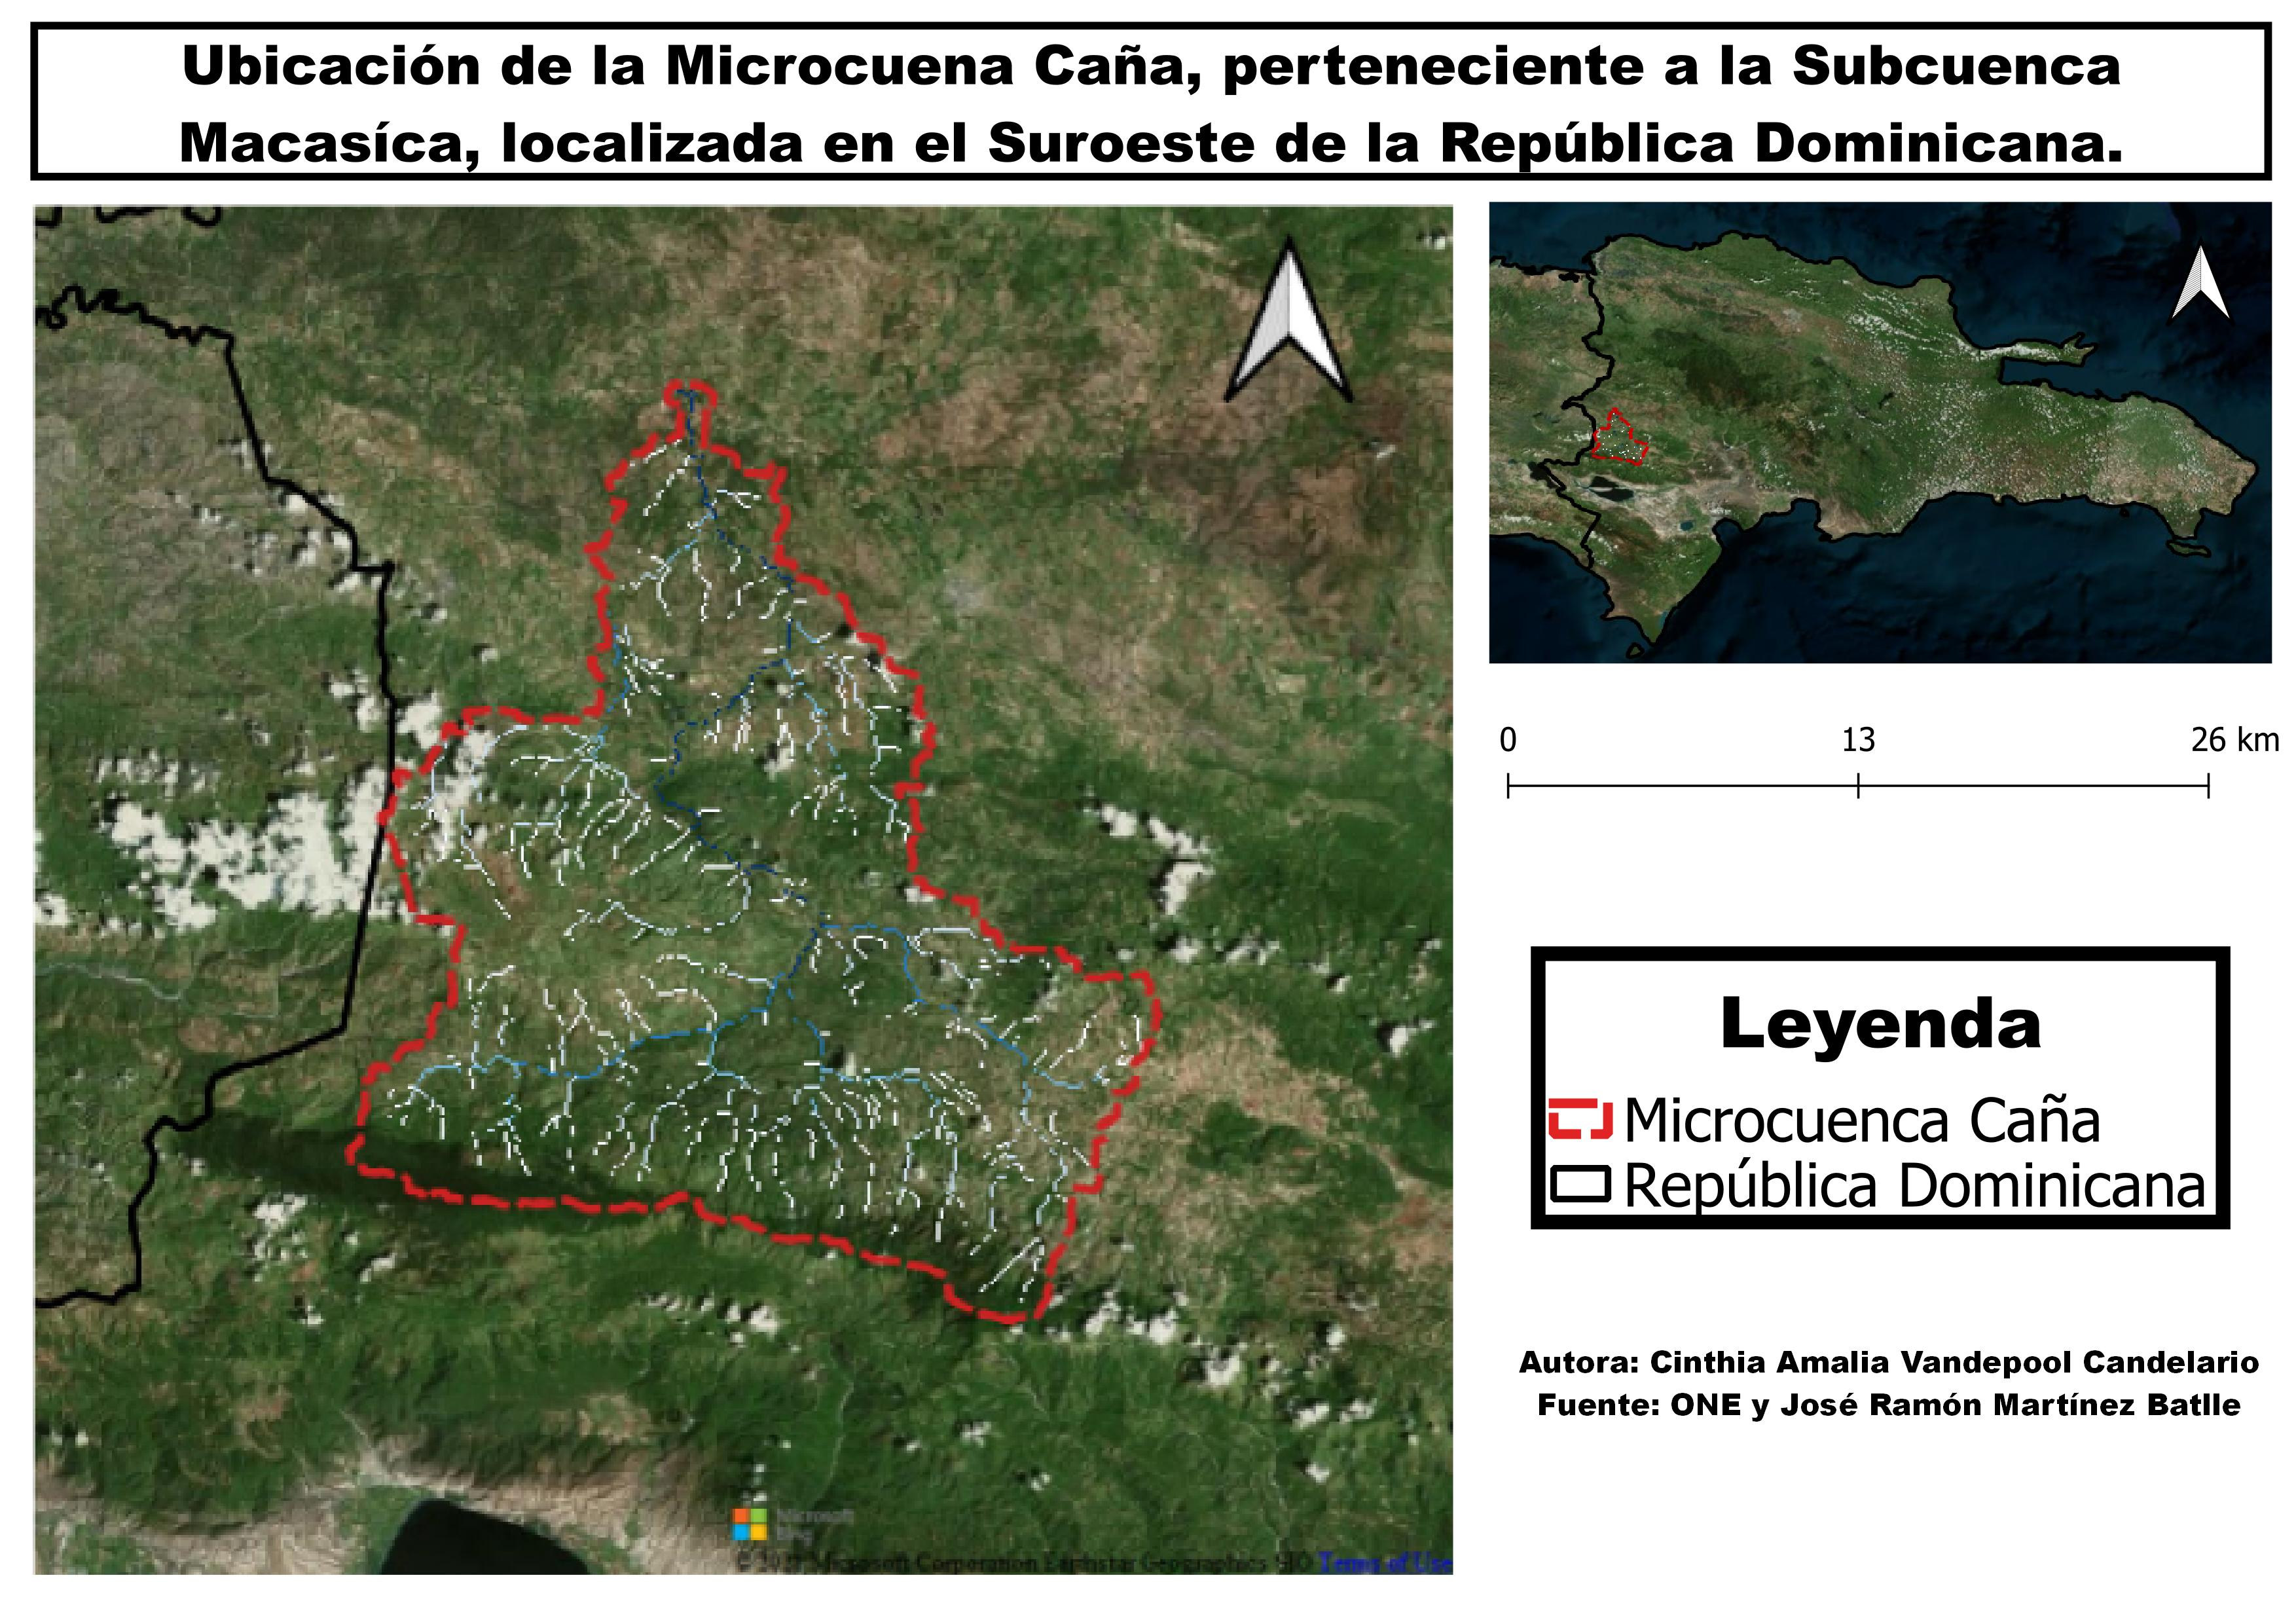
\includegraphics[width=0.75000\textwidth]{mapa_de_microcuenca_cana.jpg}
\caption{Ubicación Microcuenca del Rio Caña\label{mapacuenca}}
\end{figure}

De acuerdo al mapa Zonas de Vida (OEA, 1967), la mayor superficie de la
cuenca lo ocupa el Bosque húmedo subtropical, se caracteriza por
presentar topografía que varía desde plana hasta accidentada con un
patrón de lluvia que varía de 1000 mm. a 2000 mm. Según la ubicación de
las áreas, la biotemperatura media anual es de 23ºC a 24ºC con una
evapotranspiración potencial estimada en promedio de 20\% menor que la
precipitación media total anual. El Bosque muy húmedo Montano Bajo es la
segunda en extensión, se caracteriza por la presencia de escarchas
temporales, precipitaciones que alcanzar cantidades mayores a los 2,000
mm. totales anuales con una evapotranspiración potencial estimada en
promedio de 55\% menor que la precipitación media total anual, su
topografía generalmente accidentada con elevaciones que van desde los
850 hasta los 2,100 metros y en menor proporción lo ocupa el bosque
húmedo montano bajo (Ministerio de Medio ambiente y Recursos naturales
(2016)).

La mayor parte de la cuenca discurre sobre la vertiente Norte del
sistema geomorfológico de la Sierra de Neiba y en menor proporción sobre
el Valle de San juan, siendo la geología conformada, en mayor
proporción, por Caliza tipo Neiba, Marga con calcarenita tipo
sombrerito, Marga con intercalaciones de bancos de caliza arenosa,
arenisca, marga arenosa, conglomerados, conglomerados poligenico, molasa
marina y continental y arena; y en menor proporción está conformada por
caliza en bancos de espesores variables con nódulos e intercalaciones de
pedernal de color blanco-crema, depósitos fluviales, depósitos
cuaternarios indiferenciados, Basaltos, Tobas, Aglomerados y Rocas
Volcánicas Submarinas (Ministerio de Medio ambiente y Recursos naturales
(2016)) (Ver figura\ref{mapageologico})

\begin{figure}
\centering
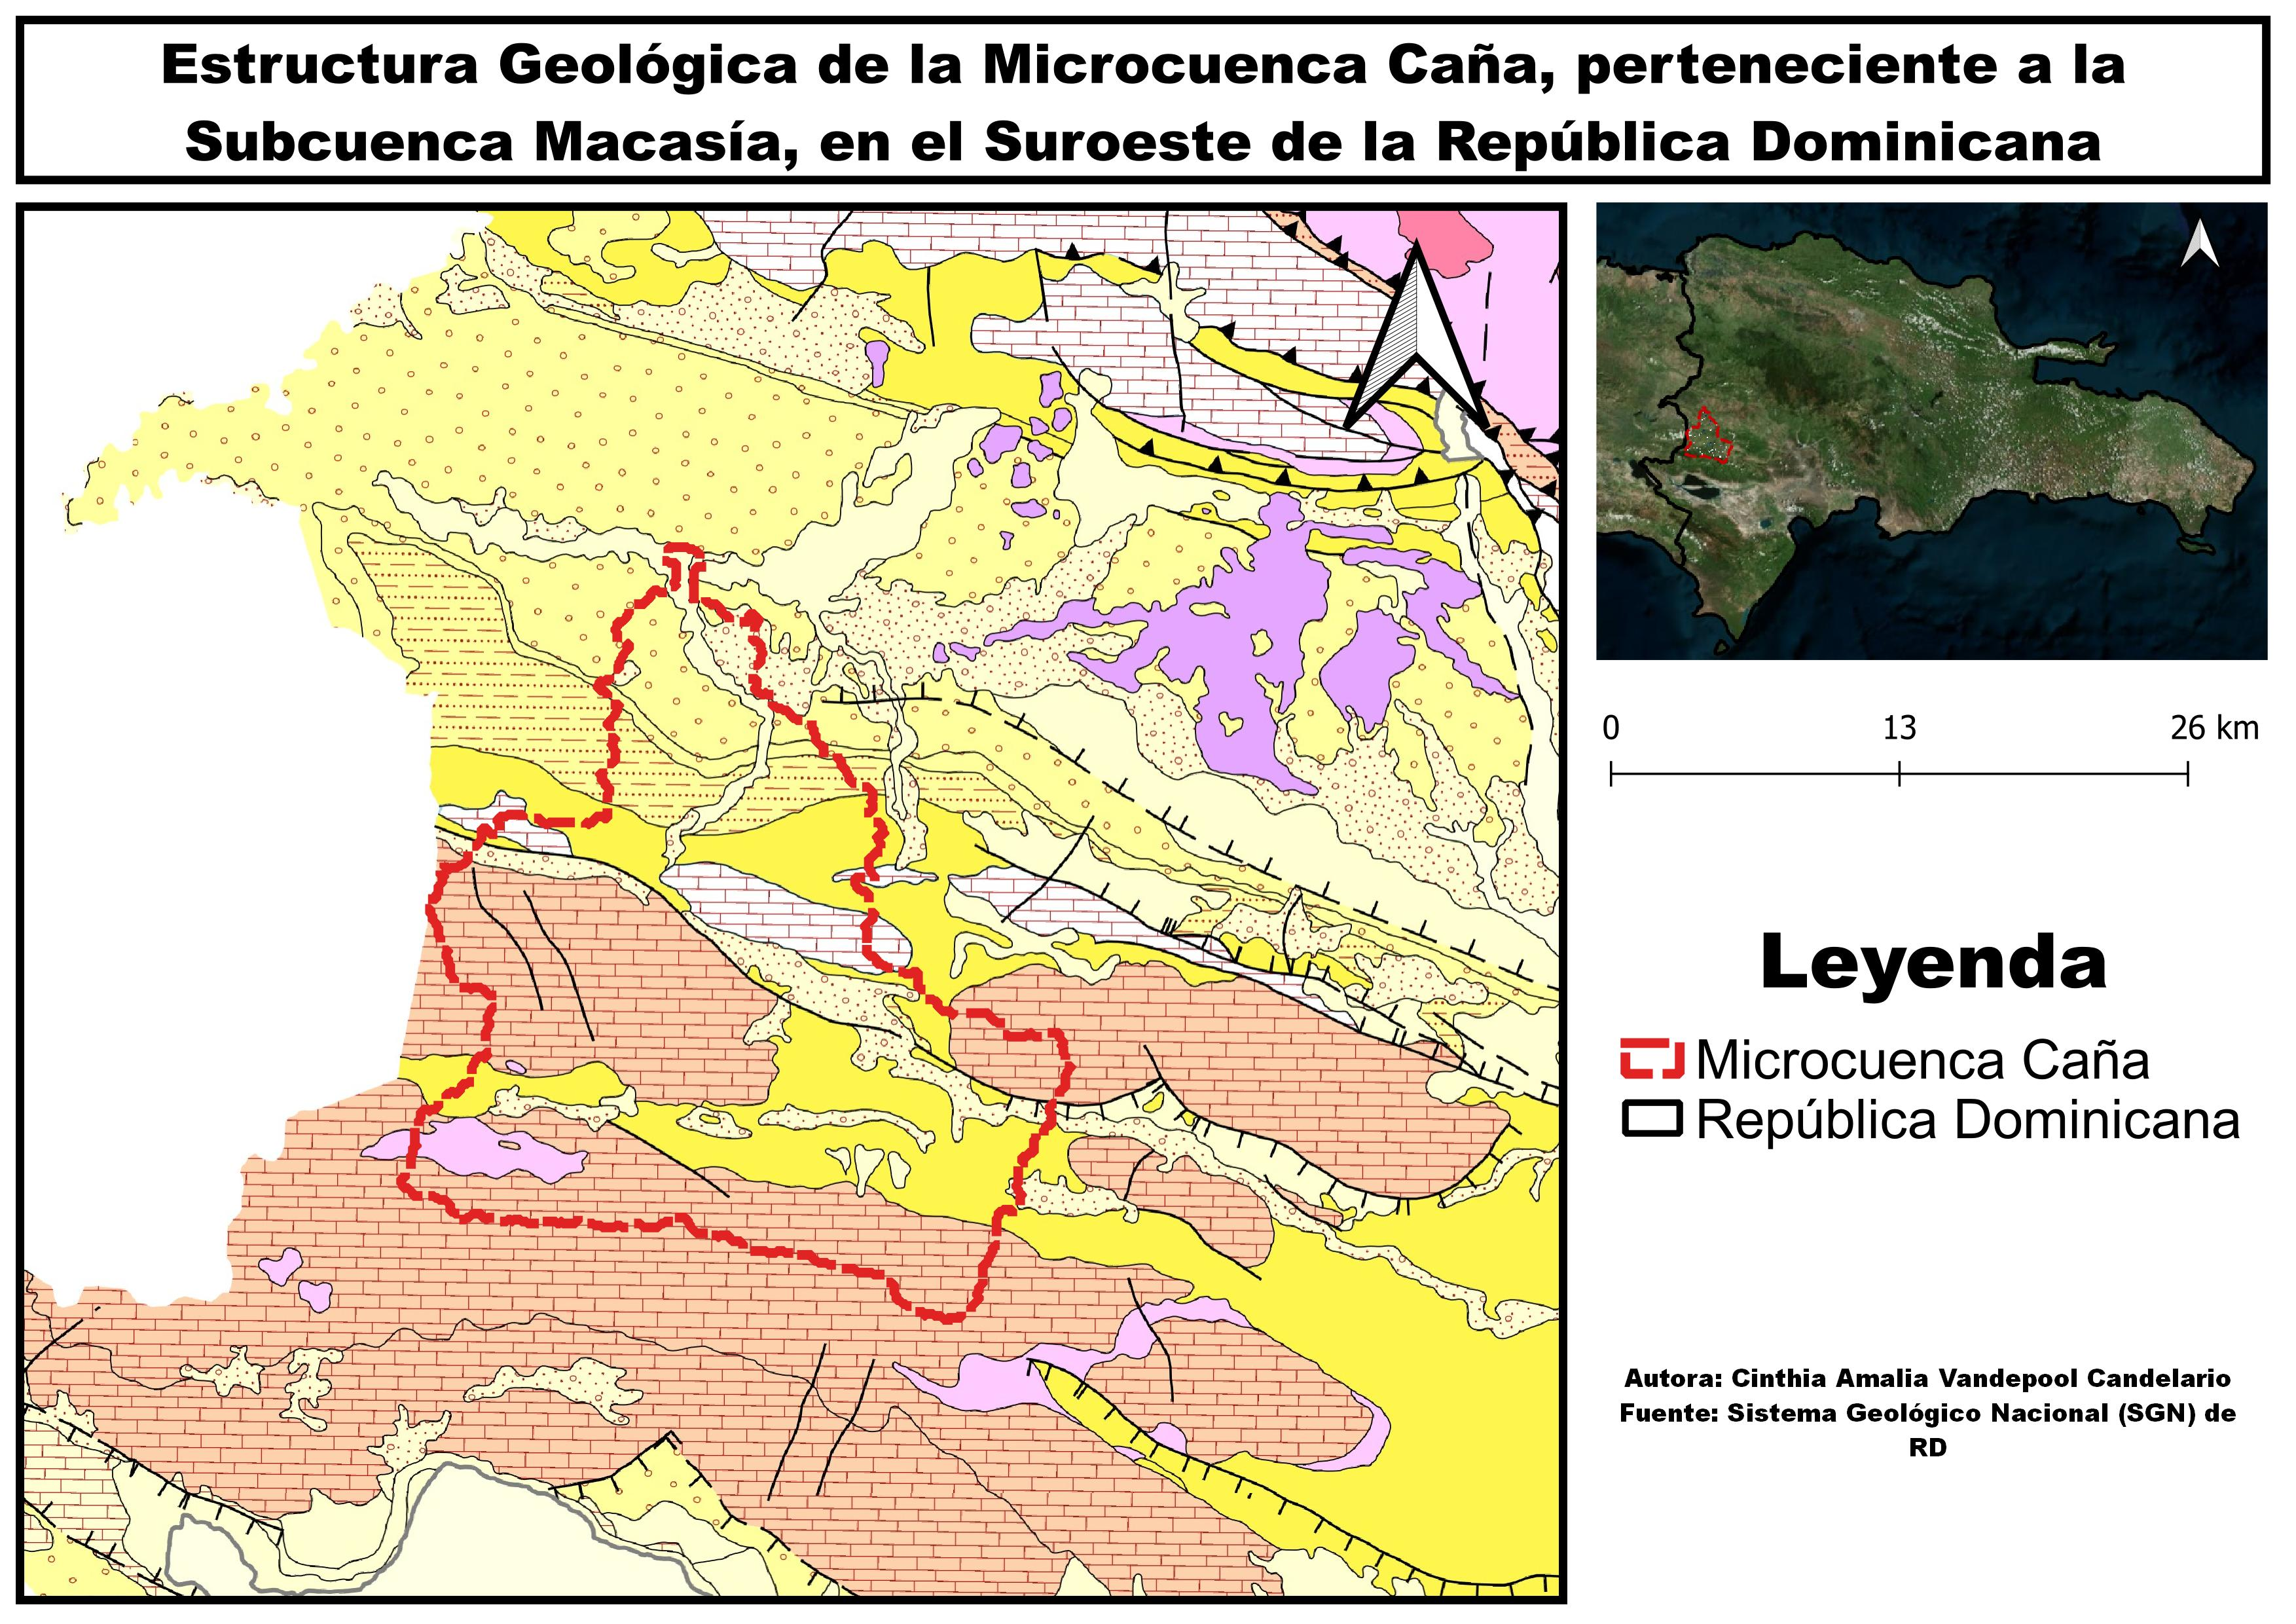
\includegraphics[width=0.75000\textwidth]{mapa_geologico_cuenca_cana.jpg}
\caption{Estructura Geológica de la Microcuenca
Caña\label{mapageologico}}
\end{figure}

\subsection{Metodología}\label{metodologuxeda-1}

Para la elaboración de esta investigación se emplearon métodos de
análisis morfométrico a partir de un DEM de la cuenca de interés,
inicialmente cargué una serie de paquetes de Grass en R adecuando el
entorno para ejecutar los códigos necesarios.

En primer lugar, se importó a R, como SpatialGridDataFrame, un DEM
alojado en la base de datos de GRASS GIS, se estableció su ruta y
convirtiéndolo a su vez en un objeto raster por medio del paquete raster
de R; partiendo del complemento \emph{r.watershed} (el cual genera un
conjunto de mapas que indican: \emph{la acumulación de flujo, la
dirección del drenaje, la ubicación de los arroyos y las cuencas
hidrográficas} (GRASS Development Team (2003g))) y del modelo digital de
elevaciones (DEM) se generaron diversas capas calculando así los
parámetros hidrográficos de la cuenca del rio caña y sus redes de
drenaje, además, seguido a esto se importó un conjunto de capas ráster
de GRASS GIS a R, como el mapa de red de drenaje y el mapa de cuencas
visualizándolas por medio de \emph{leaflet}.

Utilizando el complemento de GRASS GIS \emph{r.water.outlet} (GRASS
Development Team (2003f)) y apoyándose en los paquetes \emph{mapview}
(Tim Appelhans and others (2020)) y \emph{leaflet} se extrajo la cuenca
de drenaje a partir de un mapa de dirección de flujos con un umbral de
acumulación de \emph{80 celdas} y las coordenadas de la desembocadura de
la cuenca cana (-71.62524,18.94026).

Posteriormente se estableció una máscara usando el límite de la cuenca
caña para luego realizar la extracción partir del DEM de la red de
drenaje utilizando el complemento de GRASS GIS \emph{r.stream.extract}
(GRASS Development Team (2003d)) desde R. Tras esto, se utilizó el
complemento \emph{r.stream}(GRASS Development Team (2003e)) para generar
un mapa de dirección de flujo, \emph{r.stream.order} (GRASS Development
Team (2003b)) para un mapa de orden de red según varios métodos, entre
ellos el método de Strahler y de Horton, a partir de
\emph{r.stream.basins} (GRASS Development Team (2003c)) un mapa de
cuencas según órdenes de red y apoyándose del complemento
\emph{r.stream.stats}(GRASS Development Team (2003a)) se generó las
estadísticas de red resumidas por órdenes, incluyendo la razón de
bifurcación.

También obtuvimos el curso más largo de la microcuenca a partir de la
función creada por José Ramón Martínez \emph{LfpNetwork}, además con la
misma función pudimos obtener los cursos más largos de las cuencas
tributarias. Seguido generamos los perfiles longitudinales de la
microcuenca y calculamos sus índices de concavidad y a partir de las
herramientas \emph{QGIS} y \emph{Google EARTH} cruzamos la información
geológica con los patrones de concavidad/convexidad.

Luego utilizamos \emph{r.basin} para determinar los parámetros
morfométricos de la microcuenca en estudio, tales como el área de la
microcuenca, su perímetro, la pendiente, los órdenes de red, entre
otros. Y por últimos, utilizamos mapas de la microcuenca y el MDE para
crear curvas hipsométricas y calcular la integral hipsométrica
utilizando la función \emph{HypsoIntCurve} creada por José Ramón
Martínez.

\section{Resultados}\label{resultados}

\subsection{Delimitación y Forma de la
Microcuenca}\label{delimitaciuxf3n-y-forma-de-la-microcuenca}

A partir de los códigos ejecutados determinamos que la microcuenca del
rio caña posee una superficie de 525 km\textsuperscript{2} con un
perímetro de 139 km, presentando una forma similar a la de un triángulo,
presenta mayor extensión en el Sur reduciendo su extensión así el Norte.
(figura\ref{areacuenca})

\begin{figure}
\centering
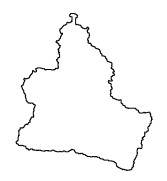
\includegraphics[width=0.30000\textwidth]{area_cana.jpg}
\caption{Área de la microcuenca\label{areacuenca}}
\end{figure}

\subsection{Datos de Elevación}\label{datos-de-elevaciuxf3n}

Esta microcuenca posee una elevación máxima de 2,231 metros sobre el
nivel del mar, una elevación mínima de 330 metros sobre el nivel del mar
y una elevación media de 958 metros. Además, presenta una pendiente de
10.56 (figura\ref{pendiente} figura\ref{mapadependiente}).

\begin{figure}
\centering
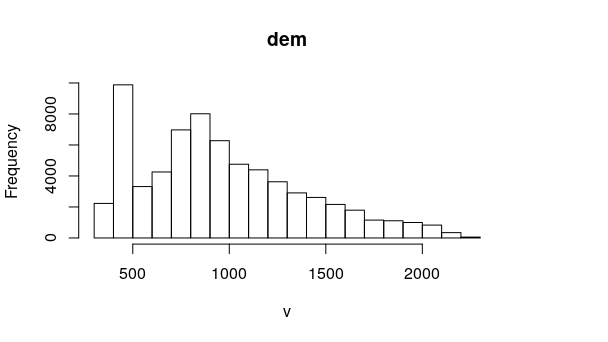
\includegraphics[width=0.50000\textwidth]{pendiente_cana.png}
\caption{Pendiente\label{pendiente}}
\end{figure}

\begin{figure}
\centering
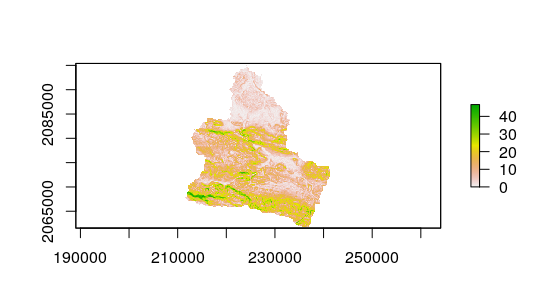
\includegraphics[width=0.50000\textwidth]{mapa_pendiente_cana.png}
\caption{Mapa de Pendiente\label{mapadependiente}}
\end{figure}

\subsection{Red de Drenaje, Orden de Red y Razón de
Bifurcación}\label{red-de-drenaje-orden-de-red-y-razuxf3n-de-bifurcaciuxf3n}

Partiendo del complemento \emph{r.stream} se generó la red de drenaje de
la microcuenca caña y utilizando el método de Strahler se determinó el
orden de red siendo el orden máximo de 5. En total la cuenca tiene 271
cursos de fluviales y una densidad de drenaje de 0.84
km/km\textsuperscript{2} (figura\ref{reddrenaje}).

\begin{figure}
\centering
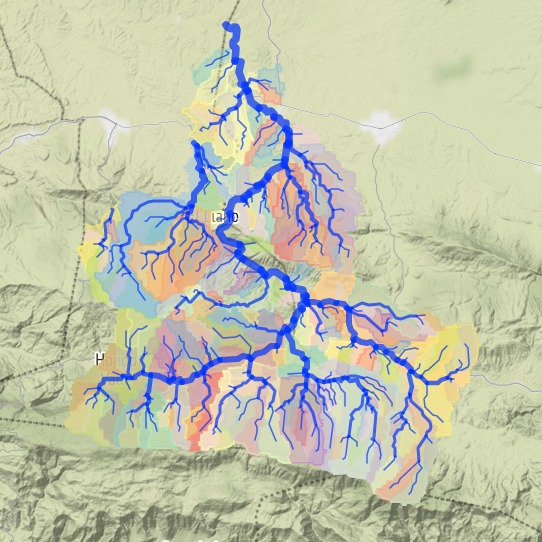
\includegraphics[width=0.57000\textwidth]{mapa_orden_de_red.jpeg}
\caption{Red de drenaje de la Microcuenca Caña\label{reddrenaje}}
\end{figure}

\begin{longtable}[]{@{}cc@{}}
\toprule
Orden de Red & No. de Cursos fluviales\tabularnewline
\midrule
\endhead
1 & 204\tabularnewline
2 & 50\tabularnewline
3 & 12\tabularnewline
4 & 4\tabularnewline
5 & 1\tabularnewline
\bottomrule
\end{longtable}

A continuación, se indicarán la razón de bifurcación de todos los
órdenes de red de la microcuenca caña, utilizando dos procedimientos
distintos:

La razón de bifurcación promedio del par de ordenes 1\textbar{}2 es
204/50=4.08, para el par de ordenes 2\textbar{}3 es 50/12=4.16, para el
par de ordenes 3\textbar{}4 es 12/4=3 y para el par de ordenes
4\textbar{}5 es 4/1=4; el valor promedio es Rb= 3.811667. Mientras la
razón de bifurcación por medio de coeficientes de regresión es Rb=
3.7292 (figura\ref{razonbifurcacion}).

\begin{figure}
\centering
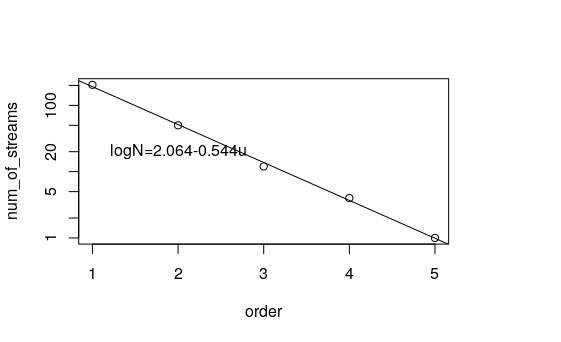
\includegraphics{razon_de_bifurcacion.png}
\caption{Recta de regresión para el modelo ``número de cursos fluviales
es función del orden de red'' y ecuación
correspondiente\label{razonbifurcacion}}
\end{figure}

\subsubsection{Perfiles Longitudinales e Índices de
Concavidad}\label{perfiles-longitudinales-e-uxedndices-de-concavidad}

EL curso más largo discurre por el lado occidental de la cuenca y posee
una longitud de 58.1 Kilometros (figura\ref{cursolargo}).

\begin{figure}
\centering
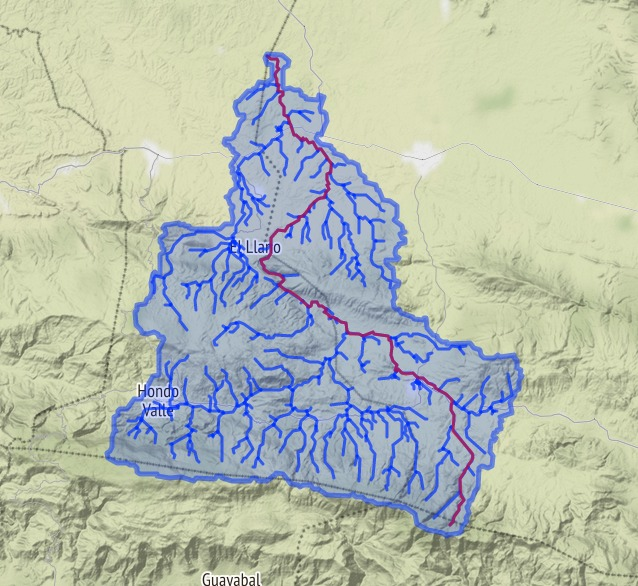
\includegraphics{curso_mas_largo.jpeg}
\caption{Curso fluvial más largo de la Microcuenca
Caña\label{cursolargo}}
\end{figure}

Según los resultados obtenidos, en su mayoria los cursos de la
microcuenca presentan un perfil concavo y en pocas ocasiones pesenta un
perfil convexo pudiendo deberese esto a estar en zona de cabecera o por
discurrir sobre depositos aluviales; además, algunos flujos presentan un
perfil rectilino que puede deberse al tipo de material por el que
discurre.

\begin{figure}
\centering
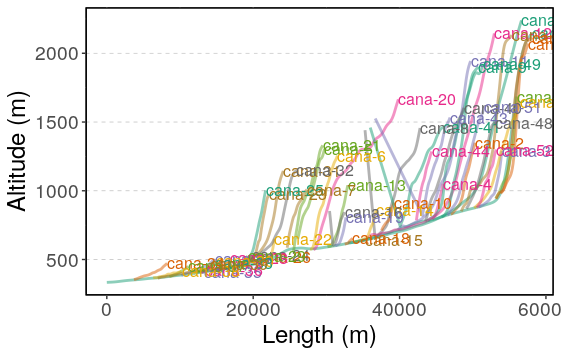
\includegraphics{perfiles_cana.png}
\caption{Perfil de Concavidad\label{perfilconcavidad}}
\end{figure}

\begin{figure}
\centering
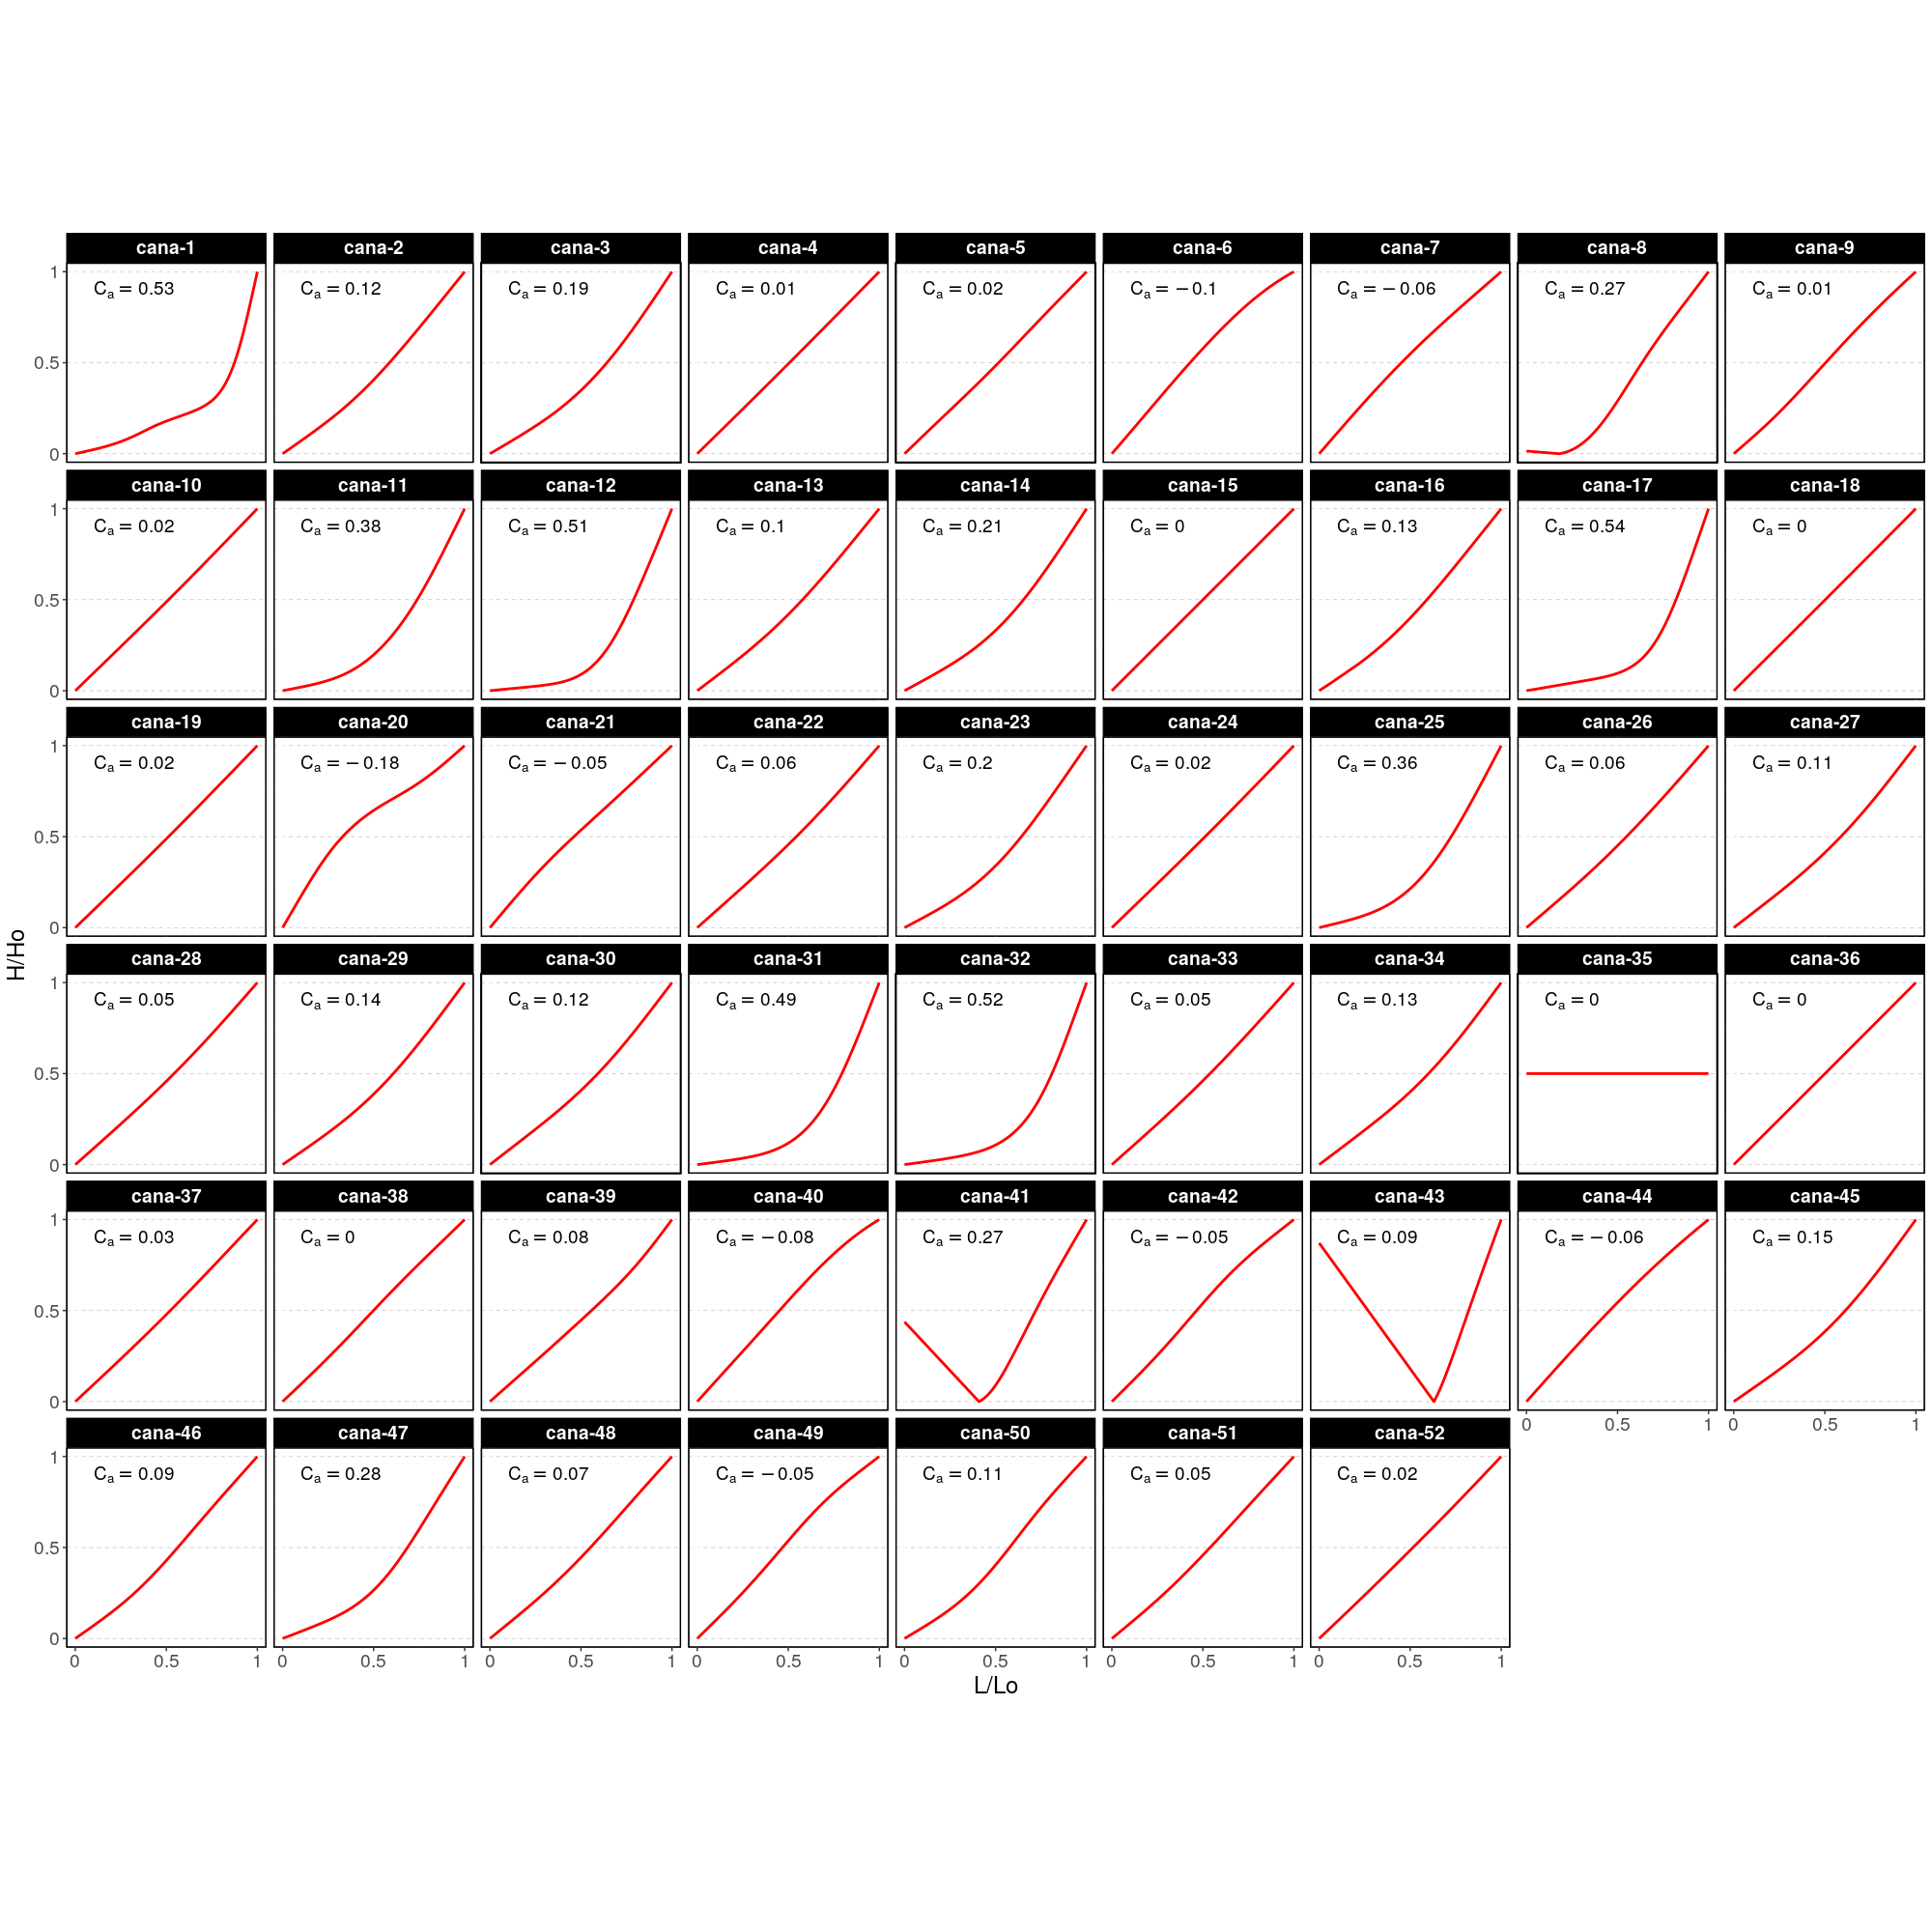
\includegraphics{indice_concavidad.png}
\caption{Indice de Concavidad\label{indiceconcavidad}}
\end{figure}

\section{Discusión}\label{discusiuxf3n}

Gracias a las investigaciones y observaciones realizadas pudimos obtener
las características morfometricas de la microcuenca caña; Pudimos
determina que las características morfometricas de la microcuenca caña
presentan un patrón de drenaje detrítico, que según Elorza (2008) se
debe a la interacción entre el flujo y los materiales erosionables.

También, superponiendo la red de drenaje sobre el mapa geológico
nacional, pudimos observar que existen la posibilidad de un proceso de
reorganizamiendo del drenaje, aunque se requieren más estudios; además
creemos que el curso principal paso por un proceso de migración lateral,
aunque también se tendría que estudiar la evolución de la microcuenca.

Con relación a la razón de bifurcación, según Horton (1945) esta razón
debe ser constante entre un par de órdenes y el otro pero en la
microcuenca de estudio esto no sucede aunque estas variaciones sean
mínimas se requerirán estudios más profundos para determinar si es
debido a las variaciones climáticas o litológicas. Además obtuvimos
valores distintos cuando calculamos la razón de bifurcación promedio y
la razón de bifurcación por medio de coeficientes de regresión aunque la
diferencia fue de apenas 0.08.

Como consecuencia de los hallazgos de esta investigación pudimos
determinar los parámetros morfométricos de esta microcuenca, sin
embargo, este trabajo solo representa la base para formular nuevas
hipótesis que requerirán nuevas investigaciones, no solo en esta
Microcuenca sino también en todos los sistemas fluviales de la isla ya
que este tipo de estudio son escasos o inexistentes.

\section{Agradecimientos}\label{agradecimientos}

\section{Información de soporte}\label{informaciuxf3n-de-soporte}

\ldots

\section{\texorpdfstring{\emph{Script}
reproducible}{Script reproducible}}\label{script-reproducible}

\ldots

\section*{Referencias}\label{referencias}
\addcontentsline{toc}{section}{Referencias}

\hypertarget{refs}{}
\hypertarget{ref-burgos2014modelos}{}
Burgos, V. H., \& Salcedo, A. P. (2014). Modelos digitales de elevación:
Tendencias, correcciones hidrológicas y nuevas fuentes de información.
\emph{Encuentro de Investigadores En Formación En Recursos Hídricos (2,
2014, Ezeiza, Buenos Aires, Argentina). Disponible En: Http://Www. Ina.
Gov. Ar/Ifrh-2014/Eje1/1.11. Pdf. Consultado}, \emph{1}(10), 2015.

\hypertarget{ref-GutierrezElorza}{}
Elorza, M. G. (2008). Geomorfologia fluvia i. In \emph{Geomorfologia}
(pp. 279--283). Pearson Educacion.

\hypertarget{ref-addonrstreamstats}{}
GRASS Development Team. (2003a). Calculates horton's statistics for
strahler and horton ordered networks created with r.stream.order.
Retrieved April 12, 2021, from
\url{https://grass.osgeo.org/grass78/manuals/addons/r.stream.stats.html}

\hypertarget{ref-addonrstreamorder}{}
GRASS Development Team. (2003b). Calculates strahler's and more streams
hierarchy. Retrieved April 12, 2021, from
\url{https://grass.osgeo.org/grass78/manuals/addons/r.stream.order.html}

\hypertarget{ref-addonrstreambasins}{}
GRASS Development Team. (2003c). Delineates basins according stream
network. Retrieved April 12, 2021, from
\url{https://grass.osgeo.org/grass78/manuals/addons/r.stream.basins.html}

\hypertarget{ref-addonrstreamextract}{}
GRASS Development Team. (2003d). Performs stream network extraction.
Retrieved April 12, 2021, from
\url{https://grass.osgeo.org/grass78/manuals/r.stream.extract.html}

\hypertarget{ref-addonrstream}{}
GRASS Development Team. (2003e). R.stream.* modules. Retrieved April 12,
2021, from \url{https://grasswiki.osgeo.org/wiki/R.stream.*_modules}

\hypertarget{ref-addonrwateroutlet}{}
GRASS Development Team. (2003f). R.water.outlet - creates watershed
basins from a drainage direction map. Retrieved April 2, 2021, from
\url{https://grass.osgeo.org/grass78/manuals/r.water.outlet.html}

\hypertarget{ref-addonrwater}{}
GRASS Development Team. (2003g). R.watershed - calculates hydrological
parameters and rusle factors. Retrieved April 2, 2021, from
\url{https://grass.osgeo.org/grass76/manuals/r.watershed.html}

\hypertarget{ref-ibanez2011morfologia}{}
Ibañez Asensio, S., Moreno Ramón, H., \& Gisbert Blanquer, J. M. (2011).
\emph{Morfología de las cuencas hidrológicas}.

\hypertarget{ref-lux2016conceptos}{}
Lux Cardona, B. (2016). \emph{Conceptos básicos de morfometría de
cuencas hidrográficas}.

\hypertarget{ref-MedioAmbiente}{}
Ministerio de Medio ambiente y Recursos naturales. (2016). Macasía.
Retrieved April 28, 2021, from
\url{https://ambiente.gob.do/cuencas-hidrograficas/macasia/}

\hypertarget{ref-mapview}{}
Tim Appelhans and others. (2020). Mapview: Interactive viewing of
spatial data in r. Retrieved April 12, 2021, from
\url{https://cran.r-project.org/web/packages/mapview/index.html}




\newpage
\singlespacing 
\end{document}
